\documentclass[dvipdfmx]{standalone}
\usepackage{tikz}

\begin{document}

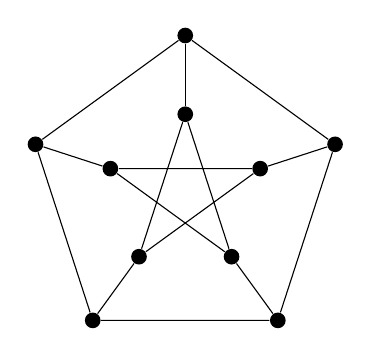
\begin{tikzpicture}[>=latex]
    \def\R{2.0}
    \def\r{1.0}
    \tikzset{dot/.style={circle, fill=black, inner sep=2pt}}
    \foreach \i in {0,...,4} {
        \node[dot] (v\i) at (90 - \i*72 : \R) {};
        \node[dot] (u\i) at (90 - \i*72 : \r) {};
    }

    \draw (v0) -- (v1) -- (v2) -- (v3) -- (v4) -- (v0);
    \draw (u0) -- (u2) -- (u4) -- (u1) -- (u3) -- (u0);
    \foreach \i in {0,...,4} {
        \draw (v\i) -- (u\i);
    }

\end{tikzpicture}

\end{document}